\section{Com\-Object\_\-MPI Class Reference}
\label{classComObject__MPI}\index{ComObject_MPI@{ComObject\_\-MPI}}
{\tt \#include $<$comobject\_\-mpi.hpp$>$}

Inheritance diagram for Com\-Object\_\-MPI::\begin{figure}[H]
\begin{center}
\leavevmode
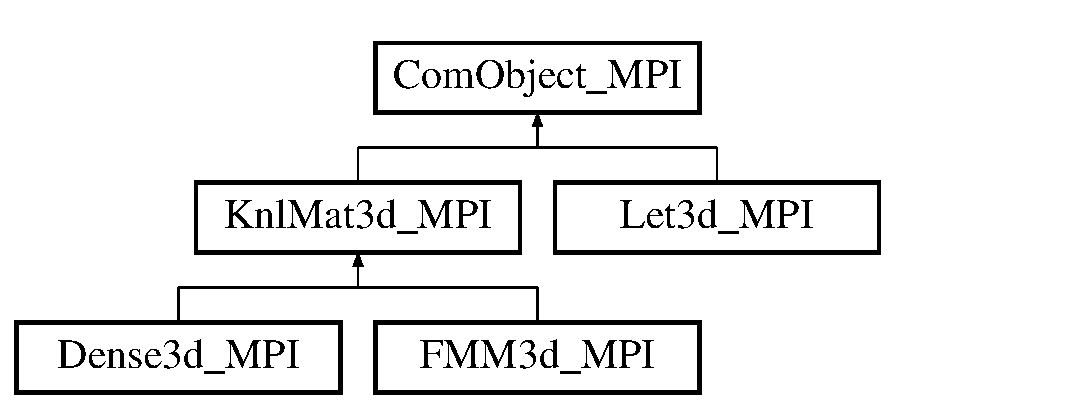
\includegraphics[height=3cm]{classComObject__MPI}
\end{center}
\end{figure}


\subsection{Detailed Description}
Com\-Object\_\-MPI class for communication purposes. Com\-Object stores basic message passing interface (mpi) information such as size and rank as defined in files included from using petsc $\ast$/. 



Definition at line 28 of file comobject\_\-mpi.hpp.\subsection*{Public Member Functions}
\begin{CompactItemize}
\item 
{\bf Com\-Object\_\-MPI} (const string \&prefix)
\item 
virtual {\bf $\sim$Com\-Object\_\-MPI} ()
\item 
const string \& {\bf prefix} ()
\item 
const MPI\_\-Comm \& {\bf mpi\-Comm} () const 
\item 
int {\bf mpi\-Rank} () const 
\item 
int {\bf mpi\-Size} () const 
\end{CompactItemize}
\subsection*{Protected Attributes}
\begin{CompactItemize}
\item 
string {\bf \_\-prefix}
\end{CompactItemize}


\subsection{Constructor \& Destructor Documentation}
\index{ComObject_MPI@{Com\-Object\_\-MPI}!ComObject_MPI@{ComObject\_\-MPI}}
\index{ComObject_MPI@{ComObject\_\-MPI}!ComObject_MPI@{Com\-Object\_\-MPI}}
\subsubsection{\setlength{\rightskip}{0pt plus 5cm}Com\-Object\_\-MPI::Com\-Object\_\-MPI (const string \& {\em prefix})\hspace{0.3cm}{\tt  [inline]}}\label{classComObject__MPI_77766478bbb936b1c62d5dc2dadd6788_77766478bbb936b1c62d5dc2dadd6788}


Initialize Com\-Object using string prefix 

Definition at line 35 of file comobject\_\-mpi.hpp.

\footnotesize\begin{verbatim}35 : _prefix(prefix) {;}
\end{verbatim}\normalsize 


\index{ComObject_MPI@{Com\-Object\_\-MPI}!~ComObject_MPI@{$\sim$ComObject\_\-MPI}}
\index{~ComObject_MPI@{$\sim$ComObject\_\-MPI}!ComObject_MPI@{Com\-Object\_\-MPI}}
\subsubsection{\setlength{\rightskip}{0pt plus 5cm}virtual Com\-Object\_\-MPI::$\sim$Com\-Object\_\-MPI ()\hspace{0.3cm}{\tt  [inline, virtual]}}\label{classComObject__MPI_b2929ed911fe3ec837f9654ff26a4249_b2929ed911fe3ec837f9654ff26a4249}




Definition at line 36 of file comobject\_\-mpi.hpp.

\footnotesize\begin{verbatim}36 {;}
\end{verbatim}\normalsize 




\subsection{Member Function Documentation}
\index{ComObject_MPI@{Com\-Object\_\-MPI}!mpiComm@{mpiComm}}
\index{mpiComm@{mpiComm}!ComObject_MPI@{Com\-Object\_\-MPI}}
\subsubsection{\setlength{\rightskip}{0pt plus 5cm}const MPI\_\-Comm\& Com\-Object\_\-MPI::mpi\-Comm () const\hspace{0.3cm}{\tt  [inline]}}\label{classComObject__MPI_dcb2a13b1c9df08fe9bc759bcfdb150e_dcb2a13b1c9df08fe9bc759bcfdb150e}


return MPI\_\-comm - set to PETSC\_\-COMM\_\-WORLD 

Definition at line 41 of file comobject\_\-mpi.hpp.

\footnotesize\begin{verbatim}41 { return PETSC_COMM_WORLD; }
\end{verbatim}\normalsize 


\index{ComObject_MPI@{Com\-Object\_\-MPI}!mpiRank@{mpiRank}}
\index{mpiRank@{mpiRank}!ComObject_MPI@{Com\-Object\_\-MPI}}
\subsubsection{\setlength{\rightskip}{0pt plus 5cm}int Com\-Object\_\-MPI::mpi\-Rank () const\hspace{0.3cm}{\tt  [inline]}}\label{classComObject__MPI_ae51fcdfaec9ca26c842280cf6b99aa9_ae51fcdfaec9ca26c842280cf6b99aa9}


return rank (id) of MPI\_\-Comm\_\-rank of PETSC\_\-COMM\_\-WORLD 

Definition at line 43 of file comobject\_\-mpi.hpp.

Referenced by Let3d\_\-MPI::print().

\footnotesize\begin{verbatim}43 { int rank; MPI_Comm_rank(PETSC_COMM_WORLD, &rank); return rank; }
\end{verbatim}\normalsize 


\index{ComObject_MPI@{Com\-Object\_\-MPI}!mpiSize@{mpiSize}}
\index{mpiSize@{mpiSize}!ComObject_MPI@{Com\-Object\_\-MPI}}
\subsubsection{\setlength{\rightskip}{0pt plus 5cm}int Com\-Object\_\-MPI::mpi\-Size () const\hspace{0.3cm}{\tt  [inline]}}\label{classComObject__MPI_1cb28464592687ed96a57c17cd3e0773_1cb28464592687ed96a57c17cd3e0773}


return size of MPI\_\-Comm\_\-size of PETSC\_\-COMM\_\-WORLD 

Definition at line 45 of file comobject\_\-mpi.hpp.

Referenced by FMM3d\_\-MPI::check().

\footnotesize\begin{verbatim}45 { int size; MPI_Comm_size(PETSC_COMM_WORLD, &size); return size; }
\end{verbatim}\normalsize 


\index{ComObject_MPI@{Com\-Object\_\-MPI}!prefix@{prefix}}
\index{prefix@{prefix}!ComObject_MPI@{Com\-Object\_\-MPI}}
\subsubsection{\setlength{\rightskip}{0pt plus 5cm}const string\& Com\-Object\_\-MPI::prefix ()\hspace{0.3cm}{\tt  [inline]}}\label{classComObject__MPI_8171d0694121d77c4bfba18e5745faa9_8171d0694121d77c4bfba18e5745faa9}


Return \_\-prefix string 

Definition at line 39 of file comobject\_\-mpi.hpp.

References \_\-prefix.

Referenced by Let3d\_\-MPI::setup(), and FMM3d\_\-MPI::setup().

\footnotesize\begin{verbatim}39 { return _prefix; }
\end{verbatim}\normalsize 




\subsection{Member Data Documentation}
\index{ComObject_MPI@{Com\-Object\_\-MPI}!_prefix@{\_\-prefix}}
\index{_prefix@{\_\-prefix}!ComObject_MPI@{Com\-Object\_\-MPI}}
\subsubsection{\setlength{\rightskip}{0pt plus 5cm}string {\bf Com\-Object\_\-MPI::\_\-prefix}\hspace{0.3cm}{\tt  [protected]}}\label{classComObject__MPI_b933f996cea3f524cf1514eb8539edfa_b933f996cea3f524cf1514eb8539edfa}


\_\-prefix is a string such as \char`\"{}fmm3d\_\-\char`\"{} which describes the type of object this is 

Definition at line 32 of file comobject\_\-mpi.hpp.

Referenced by prefix().

The documentation for this class was generated from the following file:\begin{CompactItemize}
\item 
fmm3d\_\-mpi/{\bf comobject\_\-mpi.hpp}\end{CompactItemize}
